Previous work on center embeddings has shown that the difficulty of doubly-nested center embeddings (akin to the \textsc{Three} condition) manifests itself not only in word-by-word reading times, but also in offline ratings.
Here, the finding is that ungrammatical versions where the second-to-last verb is missing are perceived as relatively acceptable, sometimes even more acceptable than the full, grammatical version \citep{frazier1985syntactic,gibson1999memory,Christiansen2009AUA,Gimenes2009WhenAM,Frank2018JudgementsAD}. 
For instance, (\ref{ex:ungramm}) is perceived as at least as acceptable than (\ref{ex:gramm}), even though it is ungrammatical, an effect known as \emph{structural forgetting}, a kind of \emph{grammaticality illusion} \citep{frazier1985syntactic, gibson1999memory}:

\begin{enumerate}
	\item\label{ex:gramm} The patient who the nurse who the clinic had hired admitted met the doctor.
	\item\label{ex:ungramm} The patient who the nurse who the clinic had hired met the doctor.
\end{enumerate}
It is generally accepted that the structural forgetting effect reflects processing difficulty on the third verb in (1) due to premature attachment of the second-to-last verb to the first noun \citep{gibson1999memory,lewis2005activation}, corresponding to the behavior of the posterior in Resource-Rational Lossy-Context Surprisal discussed in the main paper.
Thus, one should expect that Embedding Bias modulates the ratings difference between (1)-like and (2)-like sentences, such that humans prefer grammatical versions more strongly when Embedding Bias is higher.
Such a prediction is not made by existing accounts of the forgetting effect, but is an immediate consequence of our model.

Here, we report offline ratings studies comparing grammatical and ungrammatical versions of the \textsc{Three} condition, in an experimental setup closely following prior work on center embeddings \citep{gibson1999memory}, finding that ratings indeed exhibit the predicted effect.


\subsection{Ratings Study S1}


As in Experiments 1--2, trials paired items with nouns.
Each item had two conditions, where the \textsc{Ungrammatical} condition is obtained by removing the second-to-last verb phrase:
\begin{enumerate}
\item \textsc{Grammatical}: The NOUN that the marketing whiz who the artist had hired was a fraud shocked everyone.
\item \textsc{Ungrammatical}: The NOUN that the marketing whiz who the artist had hired shocked everyone.
\end{enumerate}
For each participant, 10 nouns and items were selected from pools of 34 nouns and 20 items, matched randomly.
Critical trials were interspersed with 45 fillers, some of which included comprehension questions.
Following \citep{gibson1999memory}, participants were asked to rate the \emph{difficulty} of sentences (``How hard is this sentence to understand?'').



This experiment consists of three sub-studies with successively more items and nouns (see Section~\ref{sec:ratings-2} for a fully confirmatory replication).
In the first part (N=9), there were twelve critical items and twelve nouns, randomly matched per participant.
In the second part (N=99), the number of items was increased to  20, and the number of nouns to 21.
In the third part (N=36), the number of nouns was increased to 34.
Here, we analyze all data together.



We recruited 144 participants on Amazon Mechanical Turk.
Stimuli, code, and data are deposited in the project repository.\footnote{\url{https://gitlab.com/m-hahn/resource-rational-surprisal/-/tree/main/experiments/rating/study1}}

11\% of participants answered less than 80\% of comprehension questions correctly and were excluded from data analysis.





We analyzed the ratings using an ordinal mixed-effect regression, with brms default priors.
We entered grammaticality and the embedding bias (both centered) as fixed effects, with random effects (including all appropriate random slopes) for subjects, nouns, and items.
The effect of interest is the interaction between grammaticality and embedding bias.


Note that the stimuli in our experiments (\textsc{Three} condition) differ from those studied in most prior work on center embeddings in that ours combine a complement clause with a relative clause (SC-ORC), whereas most work has studied stacked relative clauses (ORC-ORC).
The latter kind of stacking is known to be even more difficult to comprehend than our \textsc{Three} condition, a fact that is explained by various memory-based models of processing difficulty \citep{Gibson2000TheDL, lewis2005activation}.
We thus do not expect a full reversal of acceptability ratings as observed sometimes in previous studies; instead, we expect a main effect of grammaticality modulated by an interaction with Embedding Bias.



Results are shown in Figure~\ref{fig:expt-rating1}.
There was an effect of grammaticality, such that the \textsc{Ungrammatical} versions were rated more difficult to understand ($\beta=-1.20$, 95\% CrI $[-1.59, -0.83]$).
There was no evidence for a main effect of Embedding Bias ($\beta=0.05$, 95\% CrI $[-0.04, 0.13]$).
The key interaction had the theoretically predicted sign, such that the effect of grammaticality increased as Embedding Bias increases ($\beta=-0.27$, 95\% CrI $[-0.45, -0.09]$, $P(\beta>0) = 0.0015$).
This result matches the theoretical prediction.

\begin{figure}
	\centering
    \includegraphics[width=0.48\textwidth]{../resource-rational-surprisal/experiments/rating/study1/Submiterator-master/figures/rating_understand-logodds-byNoun-LogRatio.pdf}
	\includegraphics[width=0.48\textwidth]{../resource-rational-surprisal/experiments/rating/study1/Submiterator-master/figures/posterior-histograms-main_effects.pdf}


	\caption{Ratings Study S1 (N=128). Left: By-noun mean responses in the two conditions. Right: Posterior of mixed-effects model. The key effect of theoretical interest is the interaction between grammaticality and Embedding Bias.}\label{fig:expt-rating1}
\end{figure}


\subsection{Ratings Study S2}\label{sec:ratings-2}


In Ratings Study S2, we replicated Ratings Study S1 with the following changes.
First, we simplified the items so that the second noun phrase had only one word (as in the reading time studies).
We also added 45 new fillers, and made minor changes to some fillers to address high error rates in comprehension questions in Ratings Study 1.
Fourth, some changes were made to the set of nouns to specifically include nouns with very low and very high embedding bias to maximize statistical power.

191 participants were recruited on Prolific.
One participant was excluded by the same criterion as in Experiment S1.
Stimuli, code, and data are deposited in the project repository.\footnote{\url{https://gitlab.com/m-hahn/resource-rational-surprisal/-/tree/main/experiments/rating/study2}}

Data analysis was as in Ratings Study 1.
Results are shown in Figure~\ref{fig:exp-rating2}.

The interaction was estimated as $\beta=-0.19$, 95\% CrI $[-0.31, -0.06]$, $P(\beta>0) = 0.00275$, in agreement with the first experiment.
Interestingly, the main effect of grammaticality was much stronger than in Ratings Study S1, which could be either due to the simpler stimuli or the change in participant population (Prolific vs Mechanical Turk).


\begin{figure}
	\centering
    \includegraphics[width=0.48\textwidth]{../resource-rational-surprisal/experiments/rating/study2/Submiterator-master/figures/rating_understand-logodds-byNoun-LogRatio.pdf}
	\includegraphics[width=0.48\textwidth]{../resource-rational-surprisal/experiments/rating/study2/Submiterator-master/figures/posterior-histograms-main_effects.pdf}


	\caption{Ratings Study S2 (N=191): Replication with simpler stimuli. Note that the main effect of grammaticality is stronger than with the more complex stimuli (Experiment S1A), but the size of the interaction is similar.}\label{fig:exp-rating2}
\end{figure}




